\begin{frame}{Datasets - Overview}
	\begin{table}[!t]
		\setlength{\tabcolsep}{4pt}
		\small
		\begin{center}
			\resizebox{.9\textwidth}{!}{
				\begin{tabular}{c|c|c|c|c|c|c}
					\toprule[1.5pt]
					Dataset       & \multicolumn{1}{c|}{Input type} &\multicolumn{1}{c|}{Target type} & \multicolumn{1}{c|}{Target range} & \multicolumn{1}{c|}{Bin size} & \multicolumn{1}{c|}{Max bin density} & \multicolumn{1}{c}{Min bin density} \\ \midrule\midrule
					IMDB-WIKI-DIR & Face image & Age & 0 - 186 & 1 & 7,149  & 1 \\ \midrule
					AgeDB-DIR     & Face image & Age & 0 - 101 & 1 & 353    & 1 \\ \midrule
					STS-B-DIR     & Sentence pairs & Text similarity score & 0 - 5  & 0.1 &  428  & 1 \\ \midrule
					NYUD2-DIR     & Indoor scene image & Depth map & 0.7 - 10 [m] & 0.1  &  $1.46 \times 10^8$ & $1.13 \times 10^6$ \\ \midrule
					SHHS-DIR      & PSG signals & Health condition score & 0 - 100 & 1  & 275 & 0 \\
					\bottomrule[1.5pt]
			\end{tabular}}
		\end{center}
	\end{table}
	\begin{table}[!t]
		\setlength{\tabcolsep}{4pt}
		\small
		\begin{center}
			\resizebox{0.5\textwidth}{!}{
				\begin{tabular}{c|c|c|c}
					\toprule[1.5pt]
					Dataset       & \multicolumn{1}{c|}{\# Training set} & \multicolumn{1}{c|}{\# Val. set} & \multicolumn{1}{c}{\# Test set} \\ \midrule\midrule
					IMDB-WIKI-DIR & 191,509 & 11,022 & 11,022 \\ \midrule
					AgeDB-DIR     & 12,208  & 2,140  & 2,140  \\ \midrule
					STS-B-DIR     & 5,249  &  1,000  & 1,000  \\ \midrule
					NYUD2-DIR     & 50,688 ($3.51 \times 10^9$)  & $-$ & 654 ($8.70\times 10^5$)    \\ \midrule
					SHHS-DIR      & 1,892 & 369 & 369 \\
					\bottomrule[1.5pt]
			\end{tabular}}
		\end{center}
	\end{table}
	\begin{itemize}\tiny
		\item Full-night Polysomnography (PSG) signals: Electroencephalography (EEG), Electrocardiography (ECG), and breathing signals (airflow, abdomen, and thorax).
		\item Example of an RGB image (left) and its depth map (right).
		\begin{figure}[h]
			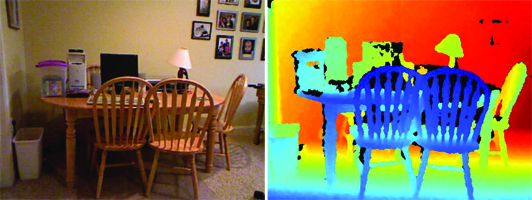
\includegraphics[width=0.5\linewidth]{images/nyu_depth_v2_raw.jpg}
		\end{figure}
	\end{itemize}
	\footlineextra{%
		\creditbase{Table}{yang2021delving}, \crediturlbase{Image}{https://cs.nyu.edu/~fergus/datasets/nyu_depth_v2.html}%
	}
\end{frame}

\begin{frame}{(Training) Datasets - Label Distributions}
	\begin{center}
		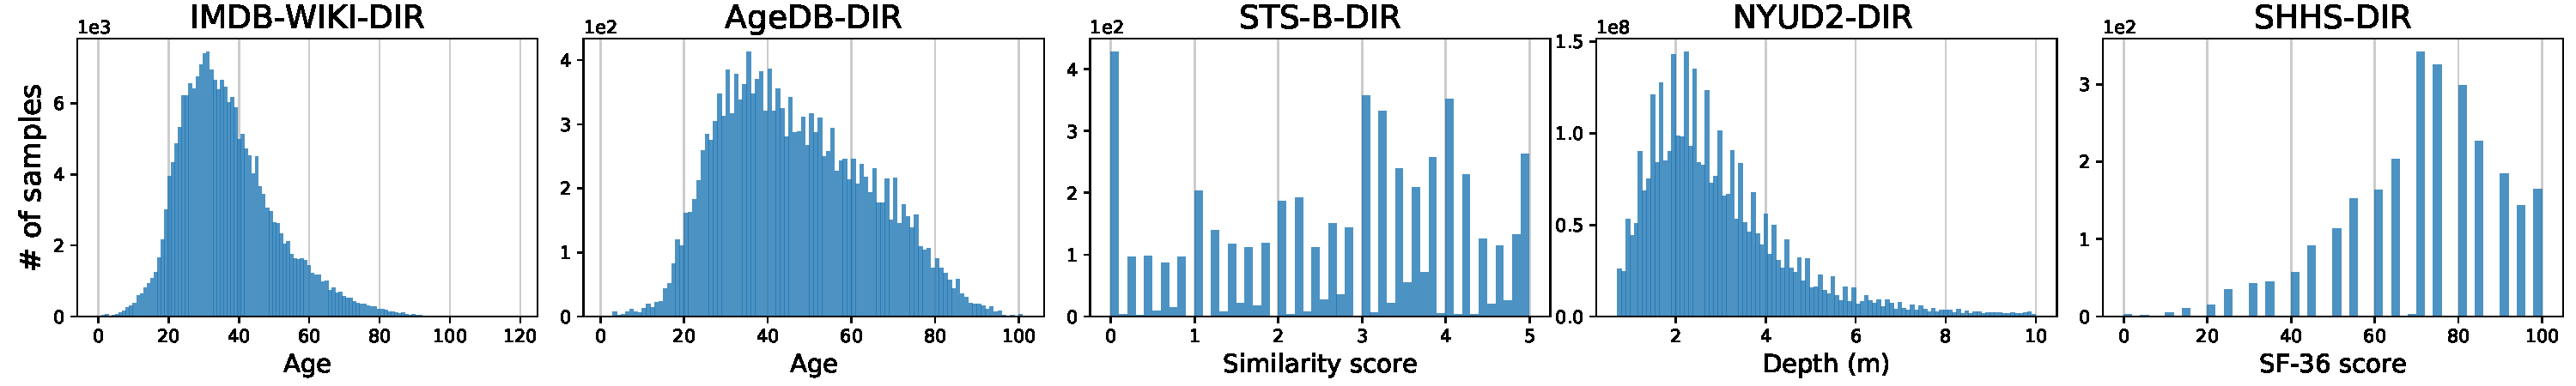
\includegraphics[trim={0 0 52em 0},clip,scale=0.4]{images/dataset_info.pdf}
		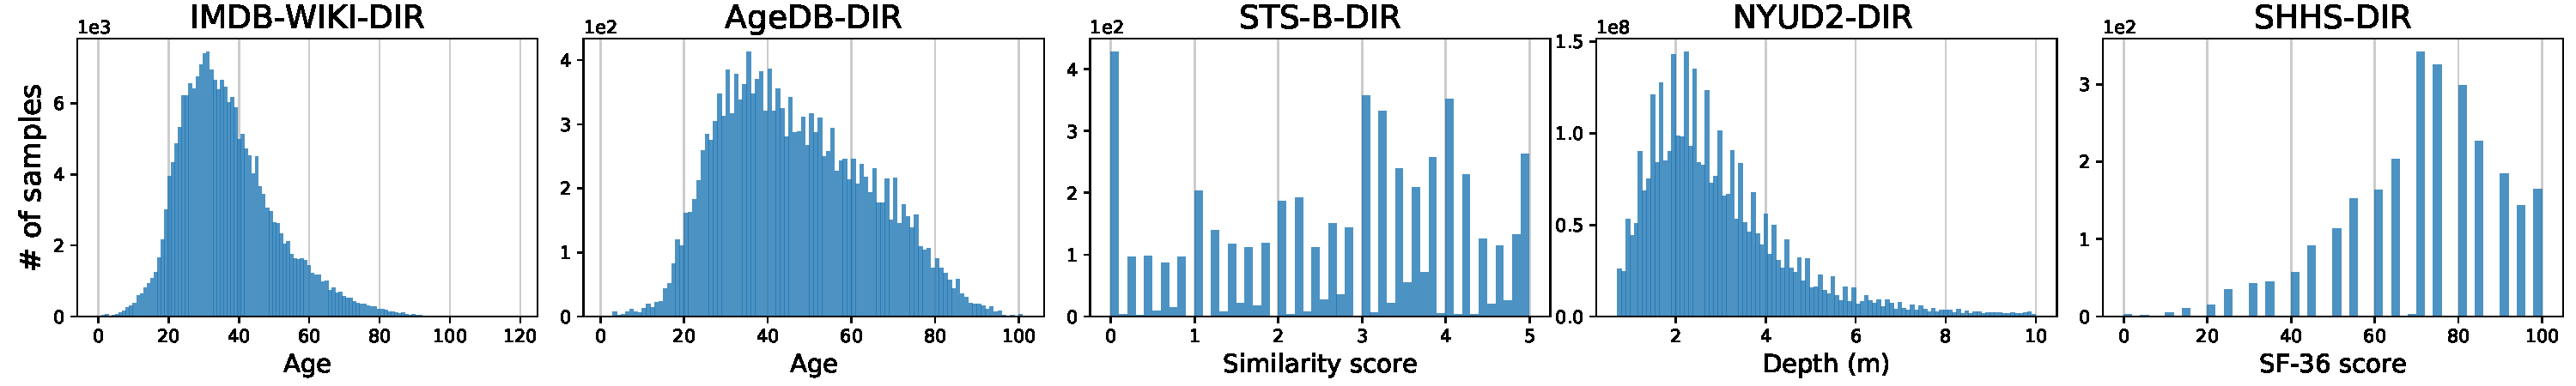
\includegraphics[trim={78.8em 0 0 0},clip,scale=0.4]{images/dataset_info.pdf}
	\end{center}
	\credit{Image}{yang2021delving}
\end{frame}